This chapter will include, for each case study: the reasoning under which that particular case study was chosen; predictions of the results; a reference to where the code for the benchmark can be found; results of the benchmark; and a discussion of the results compared to the conclusion.

\section{Specialised Benchmark, Sorting}

The first case study involves minimal allocations and a large amount of busy work.

The benchmark setup code creates input data of an array of structs containing a random value and a sequential ID (which isn't used). It then calls each of the four benchmarking functions described below a large number of times (10,000 to 20,000 times) in a row each, timing how long each execution takes in total.

The benchmarking functions each perform a single allocation before copying the input buffer into the newly allocated block. How this allocation is performed is the core difference. The four types of allocation used are described in Table~\ref{alloctype}.

Note that \functionname{alloca}\footnote{\functionname{alloca} performs a stack allocation at runtime in a similar manner to \malloc{}, but does not perform checks for whether the stack will overflow as a result and doesn't require \free{}ing as restoring the stack pointer on function return will automatically free the block} is used despite its general unsuitability for use in safe code. This is to simplify ensuring that there is always enough space in the \functionname{stack} benchmark function, in which errors are not fatal.\\
Another caveat to the use of \functionname{alloca} is that while it appears to be a standard library function, it's not actually part of the ANSI/ISO-C standard~\cite{c11std} and is simply replaced inline by compiler implementations. This causes portability concerns.

\begin{table}
	\centering
	\begin{tabularx}{\linewidth}{>{\hsize=0.6\hsize}X >{\hsize=1.4\hsize}X}
		\toprule
		\textbf{Allocation Type} & \textbf{Description} \\
		\midrule
		\functionname{malloc} & Performs the allocation with \malloc{}, providing a base performance to compare against. \free{}s the allocated block before returning \\
		\functionname{stack} & Performs the allocation with \functionname{alloca} regardless of the size of the input data even though this would introduce a significant risk of stack overflow in real code. No \free{} required \\
		\functionname{dynamic} & Performs the allocation with \malloc{} if the input data is larger than a given threshold (in this case, 64 items or 512 bytes), otherwise uses an array of static size declared as a local variable (and, hence, stack allocated as part of the calling code). \free{}s before returning if required \\
		\functionname{external} & Performs no allocation, instead taking a parameter of a pointer to a sufficiently large buffer to copy data to, which it doesn't \free{}. Acts as a control as no allocation is performed and so it should always be the fastest \\
		\bottomrule
	\end{tabularx}
	\caption{Allocation Types}\label{alloctype}
\end{table}

\subsection{Program Reasoning}

This benchmark was chosen to provide a baseline for performance changes due to application of the patch, as a minimal amount of time should be spent in allocations to be gained back by more efficient allocations.

\subsection{Predictions}

It is expected that the \functionname{external} allocation method should be fastest, as it spends no time performing allocations/deallocations. \\
The \functionname{stack} allocation method should be the next fastest, not requiring a \free{} or finding of a suitable block by \malloc{}, and should maintain a small performance increase even for larger input sizes, although this will be dwarfed by the time spent sorting. \\
\functionname{dynamic} should be roughly tied for performance with \functionname{stack} for small input sizes, thanks to not having the overhead of \functionname{alloca}, but adding the overhead of determining whether to use \malloc{} or not. It also suffers the overhead of a \free{} on exit, and should perform worse than the \functionname{malloc} allocation method on larger input sizes, but again this should be dwarfed by the time spent sorting.

\subsection{Patch Code}

Refer to the benchmark code in the \texttt{src/naive} directory in Appendix~\ref{codeappend}.

\subsection{Results}

In the diagrams in Figure~\ref{firstsort} through Figure~\ref{lastsort}, the y axis represents the time taken for a given allocation method compared to the \functionname{malloc} benchmark, while the x axis represents the size of the input data. Values below 1 on the y axis outperform \malloc{}.

The values in the diagrams are taken from a number of runs, from which the top third and bottom third of values were dropped as outliers. The minimum, maximum and mean values were then calculated from the remaining values.

\begin{figure}[ph]
	\centering
	\includegraphics[width=0.8\textwidth]{sort/O0chart}
	\caption{Unexpectedly, \functionname{stack} performs worse than \functionname{malloc}. Others perform as expected. From inspecting the generated assembly, it looks like -O0 produces very inefficient code for alloca.}\label{firstsort}
\end{figure}

\begin{figure}[ph]
	\centering
	\includegraphics[width=0.8\textwidth]{sort/O1chart}
	\caption{Everything performing mostly as expected. \functionname{stack} and \functionname{dynamic} seem to perform very similarly, until \functionname{dynamic} unexpectedly starts underperforming \functionname{malloc} shortly before falling back to \functionname{malloc} level performance at around the same input size as the other methods' performance converge with \functionname{malloc}.}
\end{figure}

\begin{figure}[ph]
	\centering
	\includegraphics[width=0.8\textwidth]{sort/O2chart}
	\caption{Everything mostly as expected. \functionname{dynamic} shouldn't be faster than \functionname{stack}, but the difference is small and the gap is closed after the first item.}
\end{figure}

\begin{figure}[ph]
	\centering
	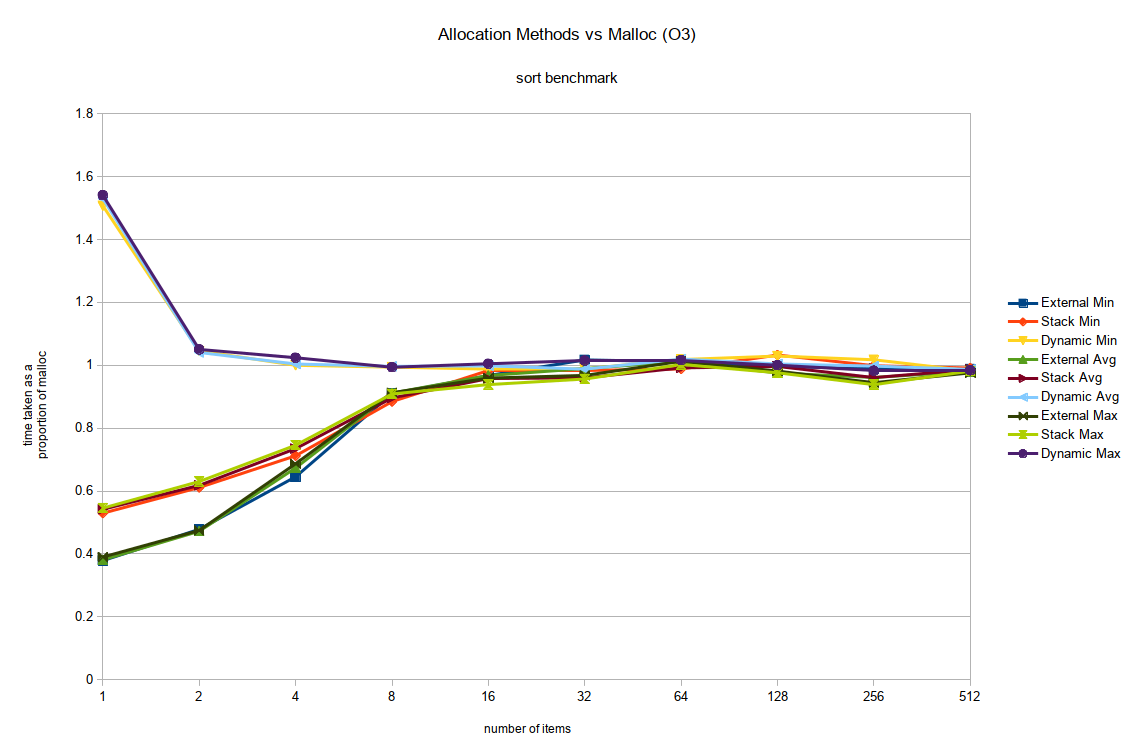
\includegraphics[width=0.8\textwidth]{sort/O3chart}
	\caption{An unusual drop of performance in the \functionname{dynamic} case, with the rest performing as expected. This appears to be caused by function inlining, where the function copying input to the allocated buffer is inlined twice in the \functionname{dynamic} benchmark function. The copy used for the case using \malloc{} is optimised to use \functionname{memcpy} while the other does not. This causes the case using stack allocation to perform worse due to the slow copy, rather than any allocation issue.}
\end{figure}

\begin{figure}[ph]
	\centering
	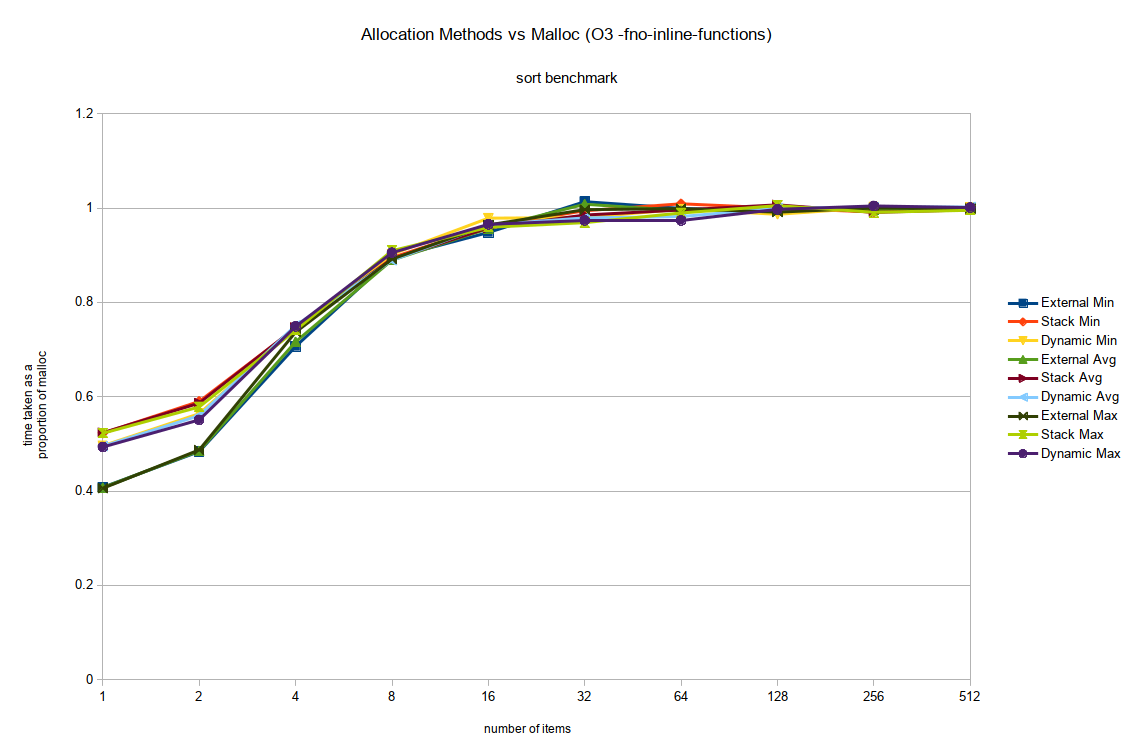
\includegraphics[width=0.8\textwidth]{sort/O3chart-no-inline}
	\caption{The same as the figure above, but with function inlining disabled. Once again, \functionname{dynamic} slightly outperforms \functionname{stack} on small cases.}\label{lastsort}
\end{figure}

\subsection{Comparison to Predictions}

Results largely matched the predictions, with the exception of \functionname{dynamic} outperforming \functionname{stack} narrowly. This may be due to the generated code for \functionname{alloca} being slower than the simple check required by the \functionname{dynamic} case.

These results bode well, especially since the lack of significant performance difference between \functionname{dynamic} and \functionname{stack} means that the safer option, \functionname{dynamic}, can be used without issue in real code.

\pagebreak

\section{Specialised Benchmark, Parallel Allocations}

The second case study involves a large number of allocations and minimal busy work.

The setup code is identical to the setup for the sort benchmark described above, but instead of calling each function a fixed number of times it sets up a number of threads (in this case 4) which all call the function simultaneously for a total of 2 seconds. This is repeated a number of times (in this case 10) and the number of times the benchmark function was successfully called is taken as an indication of performance.

However, instead of sorting the input data, the functions simply copy the input data to the allocated buffer. The allocation types used are the same as in the sort benchmark.

\subsection{Program Reasoning}

This benchmark seeks to produce a ceiling for performance increases. While there are many implementations of \malloc{}, most involve locks at some level of granularity. In particular, this benchmark was run using glibc's \malloc{}, which does take locks internally~\cite{glibcmalloc}. This benchmark seeks to maximise the contention of these locks, allowing the benchmarking functions to avoid losing time to unavailable mutexes by avoiding \malloc{}s, making them faster by comparison.

\subsection{Predictions}

The predictions are the same as in the sort benchmark, but the speed increases should be more significant.

\subsection{Patch Code}

Refer to the benchmark code in the \texttt{src/parallel} directory in Appendix~\ref{codeappend}.

\subsection{Results}

In the diagrams in Figure~\ref{firstparallel} through Figure~\ref{lastparallel}, the y axis represents the number of function calls completed for a given allocation method compared to the \functionname{malloc} benchmark, while the x axis represents the size of the input data. Values above 1 on the y axis outperform \malloc{}.

The values in the diagrams are taken from a number of runs, from which the top third and bottom third of values were dropped as outliers. The minimum, maximum and mean values were then calculated from the remaining values.

\begin{figure}[h]
	\centering
	\includegraphics[width=0.8\textwidth]{parallel/O0chart}
	\caption{\functionname{stack} performs poorly again, although this time it still outperforms \functionname{malloc}. Other allocation methods perform as predicted.}\label{firstparallel}
\end{figure}

\begin{figure}[p]
	\centering
	\includegraphics[width=0.8\textwidth]{parallel/O1chart}
	\caption{As seen in the sort benchmark, \functionname{stack} and \functionname{dynamic} perform roughly the same, while external outperforms both. Unlike the sort benchmark, \functionname{stack} and \functionname{external}'s performance benefits don't completely drop off on large input data.}
\end{figure}

\begin{figure}[p]
	\centering
	\includegraphics[width=0.8\textwidth]{parallel/O2chart}
	\caption{At this optimisation level the compiler was able to determine that the results of the copying in the benchmark functions were not being used, so the entire functions got optimised out other than the \functionname{external} method, which essentially degenerates to a \functionname{memcpy}. Higher optimisation levels yield the same result.}\label{lastparallel}
\end{figure}

\subsection{Comparison to Predictions}

Similarly to the sort benchmark, results mostly matched the predictions. As expected, performance increases were much more significant than in the sort benchmark. This is expected, as the changes made here are similar in principle to replacing a locking algorithm with a wait-free algorithm.

However, the situations in which this sort of performance increase would be possible are quite limited, as programs are not often allocating at such a high rate in parallel.

\pagebreak

\section{Real World Benchmark, \toolname{cURL} Patch}

The third and last case study involves a more careful analysis of Stenberg's patch to \toolname{cURL}~\cite{curlmalloc}. It covers both parts of the change described in Section~\ref{backgroundsec}.

The benchmark is performed by cloning \toolname{cURL}'s source and checking out\footnote{A checkout in this context refers to \texttt{git-checkout}, whereby the state of the code is rewound to a given point} the commits in which the changes were made.

In order to test the linked list changes, simply running regular \toolname{cURL} requests is enough, as indicated by the blog post. For the polling function changes, one of the code samples distributed with the \toolname{cURL} source code is modified to exercise the exact function to be benchmarked, \functionname{curl\_multi\_wait}.

\subsection{Program Reasoning}

Clearer figures for the performance impact on a real-world program were needed. The two previous benchmarks demonstrate theoretical improvements in carefully constructed scenarios, but to gain a better impression of the real-world impact, real-world code must be tested.

Since the blog post lumps in all changes from some 230 or so commits, performance impact can't be assumed to only be a result of the allocation changes. The goal of this benchmark is to isolate the changes with their effects.

\subsection{Predictions}

Given the results of the previous benchmarks and from the blog post, results are expected to be noticeable in the direction of outperforming \malloc{}, but smaller than described in the blog post.\\
This is accounting for the fact that allocations alone were unlikely to account for 30\% of the execution time as suggested in the blog post. While a large speed-up was shown in the benchmarks, they were designed primarily around allocations and took care to only measure times at the sites where allocations were changed.

By contrast, \toolname{cURL}'s timing cannot focus in only on allocation sites, and if it did focus on only the allocation sites it could miss knock-on effects from the change.

Note that the polling function, \functionname{curl\_multi\_wait}, is benchmarked with 1 and 11 file descriptors. The single file descriptor benchmark is intended to trigger the best case, where a small heap allocation is replaced with a stack allocation, whereas the 11 descriptor benchmark is intended as a control, as its performance should be identical before and after the change. This is due to the fact that only up to 10 descriptors are stack allocated.

There are a number of changes included in the linked list changes, such as: changing initialisation functions from a \malloc{}+\functionname{memset} to a single \functionname{calloc} having the same effect; or a cascading effect from the change to the linked list functions being unable to fail due to a lack of memory resulting in less checks being necessary in code using those functions. These changes could all impact the performance, but should favour the new version of the code performance-wise.\\
To test the linked list changes, a single large and empty file was retrieved from a server running locally.

\subsection{Patch Code}

Refer to the \texttt{replicate.sh} script in the \texttt{src/curl} directory in Appendix~\ref{codeappend}. Running this script on a machine with the required dependencies (refer to the \toolname{cURL} source to determine what dependencies are required to build it) will produce the executables used to benchmark and then run the benchmark.

\subsection{Results}

In the diagrams in Figure~\ref{firstcurl} through Figure~\ref{lastcurl}, the y axis represents the run-time of the patched version of \toolname{cURL} as a proportion of the time taken to perform the same task by the parent commit. This is used as a proxy for performance. On the x axis, \functionname{curl-llist} is the result of testing the linked list changes, \functionname{curl-multi-wait-1} is the result of testing the polling function changes with a single file descriptor, \functionname{curl-multi-wait-11} is the control using 11 file descriptors.

The min/avg/max times are as reported by the \toolname{time} utility, and a description of the meaning of user/real/sys is in Table~\ref{timestable}.

\begin{table}
	\centering
	\begin{tabularx}{\linewidth}{>{\hsize=0.6\hsize}X >{\hsize=1.4\hsize}X}
		\toprule
		\textbf{Time Type} & \textbf{Description} \\
		\midrule
		real & Wall clock time elapsed, i.e.\ actual time taken from the program starting to when it exits \\
		user & CPU time spent outside of kernel code \\
		sys & CPU time spent in kernel code \\
		\bottomrule
	\end{tabularx}
	\caption{Description of the meanings of times reported by \toolname{time}}\label{timestable}
\end{table}

The values in the diagrams are taken from a number of runs, from which the top third and bottom third of values were dropped as outliers. The user, real, and sys time values were then calculated from the remaining values and their minimum, maximum and mean found.

Values less than 1 outperform the parent commit.

\begin{figure}[h]
	\centering
	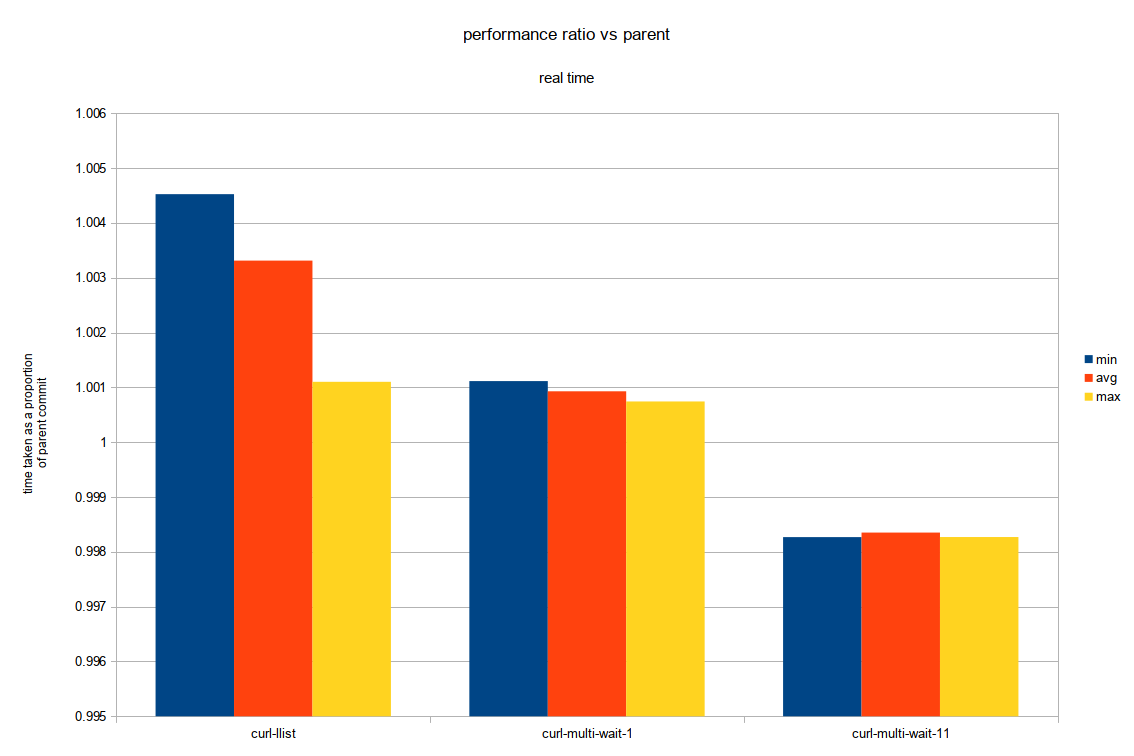
\includegraphics[width=0.8\textwidth]{curl/ratio-real}
	\caption{Nothing varies by more than 0.5\%. The only benchmark that performs better is the one that should perform identically, suggesting that any performance benefit is shadowed by other effects.}\label{firstcurl}
\end{figure}

\begin{figure}[p]
	\centering
	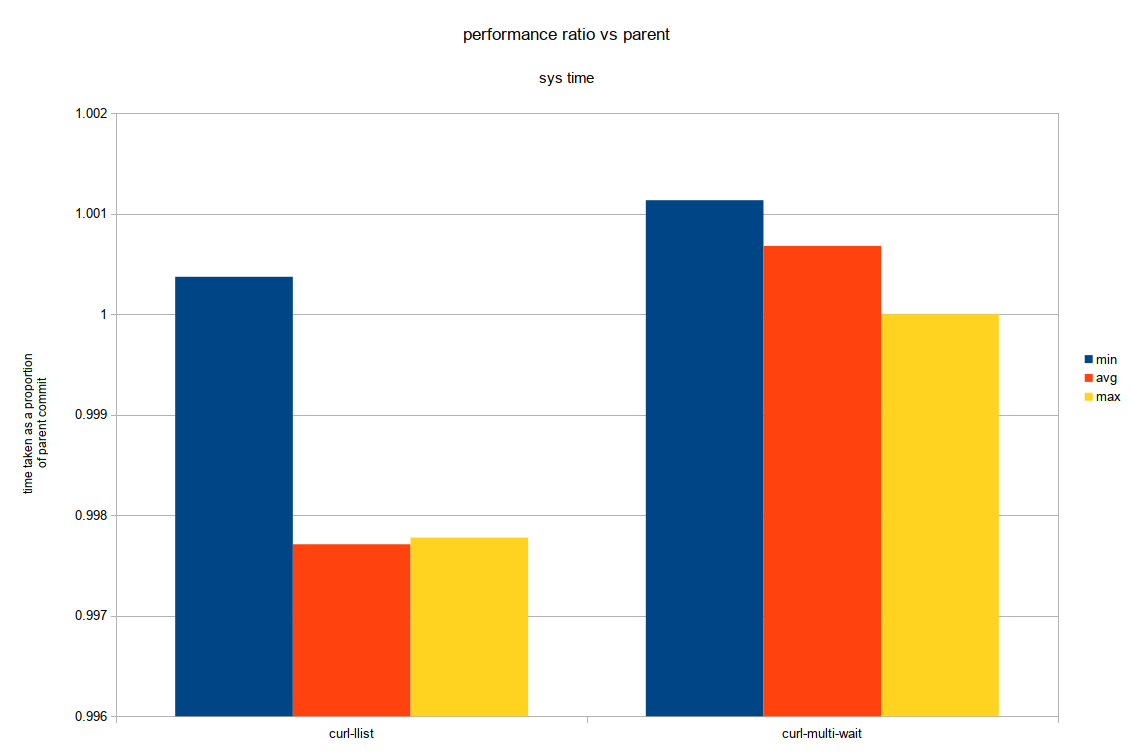
\includegraphics[width=0.8\textwidth]{curl/ratio-sys}
	\caption{sys time should in theory decrease in the first two cases, as less \malloc{}s should mean less time spent in kernel code (such as \functionname{brk}/\functionname{sbrk}/\functionname{mmap}). Once again, the maximum variation is 0.6\%, but in the wrong direction compared to predictions.}
\end{figure}

\begin{figure}[p]
	\centering
	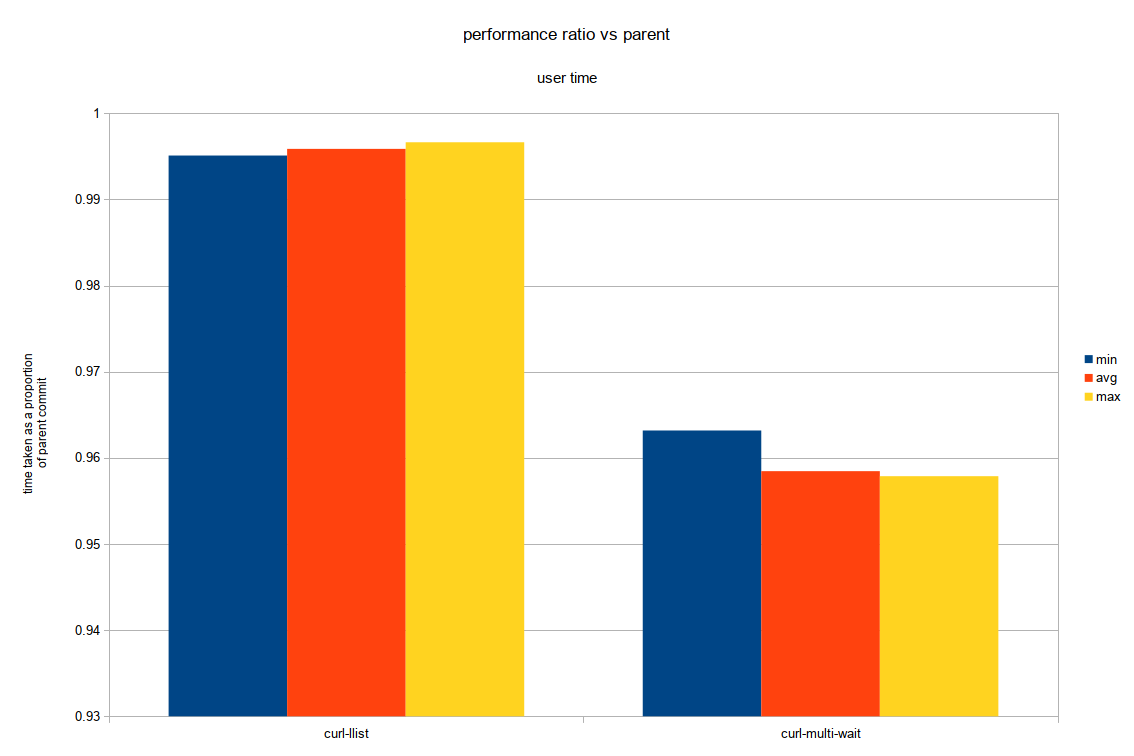
\includegraphics[width=0.8\textwidth]{curl/ratio-user}
	\caption{The llist case should decrease in time thanks to simplified code due to removal of \malloc{}s and use of more efficient library functions (\functionname{calloc} instead of \malloc{} and \functionname{memset}). For the multi-wait case, user time shouldn't really change. This is mostly met, particularly in the llist case.}\label{lastcurl}
\end{figure}

\subsection{Comparison to Predictions}

The results in this benchmark were unexpectedly poor, and differed completely from predictions and indeed from what Stenberg claimed. It seems that one or more of the other commits lumped in with his measurements may have affected the performance difference.
